\section{Domain Analysis}

\subsection{Objective of the Laboratory Work}

The objective of this laboratory work is to design, implement, and document a modular embedded control application that regulates a measurable physical parameter by means of ON-OFF control with hysteresis. The chosen individual variant is temperature control with a DHT22 digital sensor and a relay actuator. The application runs on an Arduino Mega 2560, uses FreeRTOS tasks for acquisition, control, actuation, input, and display, and reports the relevant signals to both an LCD 1602 module and the Arduino Serial Plotter.

Unlike a purely simulated laboratory exercise, this work is prepared for a real Arduino wiring setup. A Wokwi project is still included as a reproducible pin-mapping reference, but the validation evidence is expected to come from the physical circuit assembled with a DHT22 sensor, potentiometer, keypad, LCD, relay module, external load supply, LEDs, and breadboard wiring.

\subsection{Problem Definition}

\begin{quote}
\small
``Să se proiecteze și să se implementeze o aplicație modulară pentru microcontroler (MCU) care realizează controlul ON-OFF cu histereză asupra unui parametru fizic. Sistemul va acționa un actuator în funcție de valoarea măsurată a parametrului, comparată cu o valoare de referință configurabilă. Setarea valorii de referință se va face printr-un mecanism de interacțiune ales, iar valorile parametrului măsurat, ale Set Point-ului și starea actuatorului vor fi afișate pe LCD și/sau prin interfața serială. Pentru demonstrarea controlului în timp real, datele relevante (SetPoint, Value, Output) vor fi trimise către Arduino Serial Plotter.''
\end{quote}

The implemented system follows Variant A from the laboratory task. The controlled physical parameter is the ambient temperature measured by the DHT22 sensor. The relay represents a binary heating actuator: it is energized when the measured temperature falls below the lower hysteresis threshold and de-energized when the temperature rises above the upper threshold. The reference value can be set from a potentiometer or switched to manual keypad control. The keypad also supports numeric setpoint entry and hysteresis-band adjustment.

The functional requirements are the following: acquire DHT22 temperature and humidity periodically; read the potentiometer and map it to a configurable temperature setpoint; allow keypad interaction for manual setpoint mode; compute an ON-OFF control command with hysteresis; actuate the relay safely; display temperature, setpoint, thresholds, sensor validity, and relay state on the LCD; and print `SetPoint`, `Value`, `Output`, `Low`, and `High` fields in a format accepted by Arduino Serial Plotter.

The non-functional requirements are modularity, deterministic task recurrence, clear separation between drivers and application logic, reuse of existing repository libraries, preservation of previous labs, and a hardware-first validation workflow.

\subsection{Technical Requirements and Validation Criteria}

The laboratory guide requires not only an implementation, but also a clear connection between requirements and validation scenarios. For this system, the main validation question is whether the measured temperature, configurable setpoint, hysteresis thresholds, and relay command remain consistent across the LCD, Serial Plotter, and physical actuator.

\begin{table}[H]
\centering
\begin{tabular}{|p{1.0cm}|p{7.4cm}|p{5.2cm}|}
\hline
\textbf{ID} & \textbf{Requirement} & \textbf{Validation Criterion} \\
\hline
R1 & Acquire temperature and humidity from DHT22 without blocking other tasks unnecessarily. & LCD and serial output update every acquisition cycle; invalid reads set `Valid:0`. \\
\hline
R2 & Provide a configurable temperature setpoint through potentiometer and keypad. & Potentiometer changes `SetPoint`; keypad manual entry overrides it after confirmation. \\
\hline
R3 & Apply ON-OFF control with hysteresis around the selected setpoint. & Relay turns ON below \(T_{low}\), turns OFF above \(T_{high}\), and holds state inside the band. \\
\hline
R4 & Separate acquisition, control, actuation, display, and input into modules/tasks. & Source tree contains dedicated task files and reusable library modules. \\
\hline
R5 & Report SetPoint, measured Value, and Output for real-time analysis. & Arduino Serial Plotter receives named fields `SetPoint`, `Value`, and `Output`. \\
\hline
R6 & Preserve safe behavior on sensor failure. & Invalid DHT22 read forces relay command OFF and displays sensor error status. \\
\hline
\end{tabular}
\caption{Technical requirements and validation criteria}
\label{tab:requirements_validation}
\end{table}

\subsection{Used Technologies}

\subsubsection{ON-OFF Control with Hysteresis}

ON-OFF control is a binary control method that drives an actuator either fully active or fully inactive. In a temperature-control context, a heating actuator is enabled when the measured temperature is too low and disabled when the temperature has recovered. Without hysteresis, relay contacts may chatter around the setpoint because small measurement fluctuations can repeatedly cross the same threshold.

Hysteresis solves this by defining two thresholds around the setpoint. For this implementation, the lower threshold is
\[
T_{low}=SP-\frac{H}{2}
\]
and the upper threshold is
\[
T_{high}=SP+\frac{H}{2}
\]
where \(SP\) is the selected setpoint and \(H\) is the hysteresis band. The relay turns ON when \(T \leq T_{low}\), turns OFF when \(T \geq T_{high}\), and preserves its previous state between the two thresholds.

\subsubsection{DHT22 Single-Wire Sensor Interface}

The DHT22 sensor provides digital temperature and humidity measurements through a timing-based single-wire protocol. In this system, the DHT22 data line is connected to digital pin D2. The software uses the Adafruit DHT library through the reusable `DhtSensor` wrapper, which stores the last valid temperature and humidity samples and marks failed reads explicitly.

\begin{figure}[H]
\centering
\IfFileExists{resources/DomainAnalysis/UsedTechnologies/dht22_protocol.png}{%
    \includegraphics[width=0.72\textwidth]{resources/DomainAnalysis/UsedTechnologies/dht22_protocol.png}%
}{%
    \fbox{\parbox{0.70\textwidth}{\centering\color{gray}\small
        [Image pending --- save to resources/DomainAnalysis/UsedTechnologies/dht22\_protocol.png]}}%
}
\caption{DHT22 single-wire communication concept}
\label{fig:dht22_protocol}
\end{figure}

\subsubsection{I2C LCD Interface}

The LCD 1602 display uses an I2C backpack, reducing the required microcontroller wiring to SDA, SCL, 5 V, and GND. On the Arduino Mega 2560, SDA and SCL are routed to the dedicated I2C pins. The report and implementation use the same LCD address, \(0x27\), and the reusable `LcdDisplay` wrapper already present in the repository.

\begin{figure}[H]
\centering
\IfFileExists{resources/DomainAnalysis/UsedTechnologies/i2c_protocol.png}{%
    
\includegraphics[width=0.72\textwidth]{resources/DomainAnalysis/UsedTechnologies/i2c_protocol.png}%
}{%
    \fbox{\parbox{0.70\textwidth}{\centering\color{gray}\small
        [Image pending --- save to resources/DomainAnalysis/UsedTechnologies/i2c\_protocol.png]}}%
}
\caption{I2C protocol used by the LCD module}
\label{fig:i2c_protocol}
\end{figure}

\subsubsection{FreeRTOS Task Scheduling}

FreeRTOS is used to structure the application into predictable tasks. Acquisition runs every 2000 ms to respect the DHT22 sampling interval, keypad input is scanned every 50 ms, display reporting runs every 500 ms, and control and actuation are event-driven through semaphores. A mutex protects shared state between tasks.

\subsection{Hardware Components}

\subsubsection{Arduino Mega 2560}

The Arduino Mega 2560 is based on the ATmega2560 MCU. It provides enough GPIO pins for the keypad matrix, relay input, DHT22 data line, potentiometer input, and I2C LCD. The board runs at 16 MHz and provides the 5 V logic level used by the selected peripherals.

\begin{figure}[H]
\centering
\IfFileExists{resources/DomainAnalysis/HardwareComponents/arduino_mega_2560.png}{%
    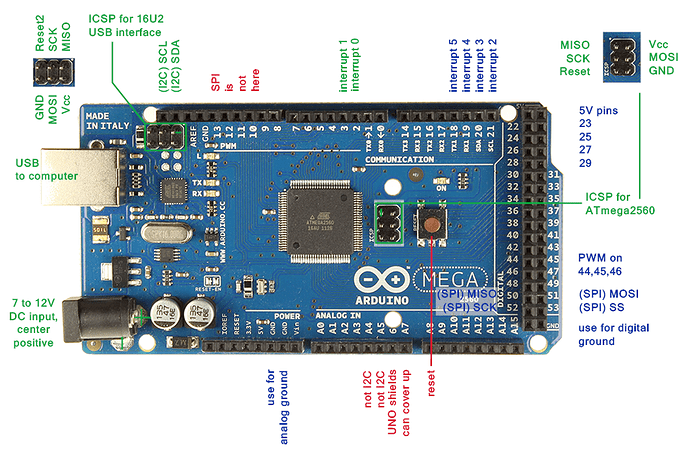
\includegraphics[width=0.62\textwidth]{resources/DomainAnalysis/HardwareComponents/arduino_mega_2560.png}%
}{%
    \fbox{\parbox{0.60\textwidth}{\centering\color{gray}\small
        [Photo pending --- save to resources/DomainAnalysis/HardwareComponents/arduino\_mega\_2560.png]}}%
}
\caption{Arduino Mega 2560 development board}
\label{fig:arduino_mega_2560}
\end{figure}

\subsubsection{DHT22 Temperature and Humidity Sensor}

The DHT22 measures ambient temperature and relative humidity. In this work, temperature is the controlled variable and humidity is displayed as diagnostic information. The sensor is powered from 5 V and its data pin is connected to D2.

\begin{figure}[H]
\centering
\IfFileExists{resources/DomainAnalysis/HardwareComponents/dht22.png}{%
    \includegraphics[width=0.45\textwidth]{resources/DomainAnalysis/HardwareComponents/dht22.png}%
}{%
    \fbox{\parbox{0.43\textwidth}{\centering\color{gray}\small
        [Photo pending --- save to resources/DomainAnalysis/HardwareComponents/dht22.png]}}%
}
\caption{DHT22 digital temperature and humidity sensor}
\label{fig:dht22}
\end{figure}

\subsubsection{Potentiometer}

The potentiometer is used as the default setpoint input. Its end terminals are connected to 5 V and GND, while the wiper is connected to A0. The ADC value is mapped to the temperature range 15--35 degrees Celsius.

\begin{figure}[H]
\centering
\IfFileExists{resources/DomainAnalysis/HardwareComponents/potentiometer.png}{%
    \includegraphics[width=0.42\textwidth]{resources/DomainAnalysis/HardwareComponents/potentiometer.png}%
}{%
    \fbox{\parbox{0.40\textwidth}{\centering\color{gray}\small
        [Photo pending --- save to resources/DomainAnalysis/HardwareComponents/potentiometer.png]}}%
}
\caption{Potentiometer used for setpoint selection}
\label{fig:potentiometer}
\end{figure}

\subsubsection{4x4 Matrix Keypad}

The keypad provides manual interaction. It allows switching between potentiometer and manual setpoint mode, increasing or decreasing the manual setpoint, entering an integer setpoint with digits, confirming with `\#`, cancelling with `*`, and cycling the hysteresis band.

\begin{figure}[H]
\centering
\IfFileExists{resources/DomainAnalysis/HardwareComponents/keypad_matrix.png}{%
    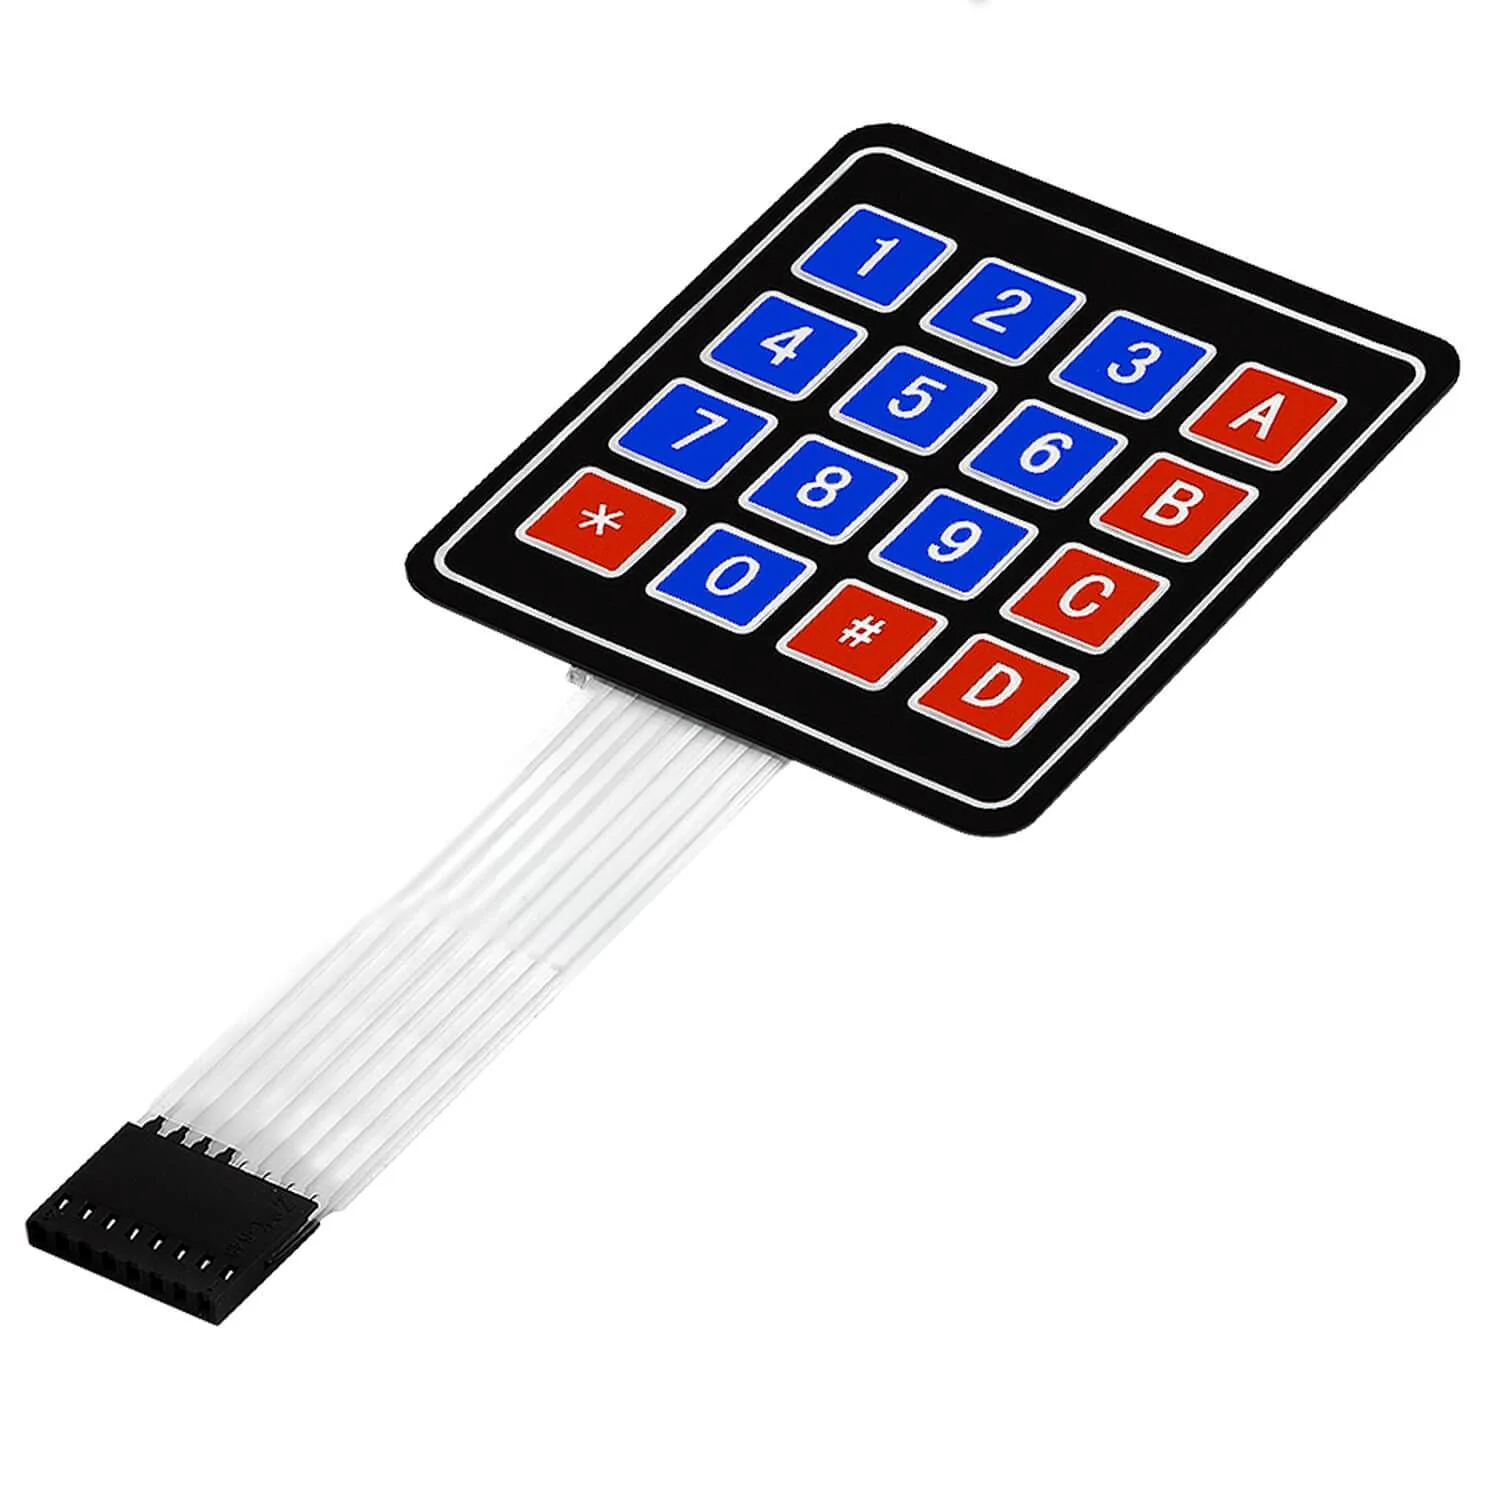
\includegraphics[width=0.45\textwidth]{resources/DomainAnalysis/HardwareComponents/keypad_matrix.png}%
}{%
    \fbox{\parbox{0.43\textwidth}{\centering\color{gray}\small
        [Photo pending --- save to resources/DomainAnalysis/HardwareComponents/keypad\_matrix.png]}}%
}
\caption{4x4 membrane matrix keypad}
\label{fig:keypad_matrix}
\end{figure}

\subsubsection{LCD 1602 I2C Display}

The LCD provides immediate feedback without a computer connection. It alternates between current control values and threshold diagnostics.

\begin{figure}[H]
\centering
\IfFileExists{resources/DomainAnalysis/HardwareComponents/lcd_1602_i2c.png}{%
    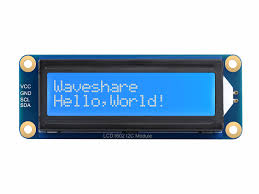
\includegraphics[width=0.50\textwidth]{resources/DomainAnalysis/HardwareComponents/lcd_1602_i2c.png}%
}{%
    \fbox{\parbox{0.48\textwidth}{\centering\color{gray}\small
        [Photo pending --- save to resources/DomainAnalysis/HardwareComponents/lcd\_1602\_i2c.png]}}%
}
\caption{LCD 1602 with I2C backpack}
\label{fig:lcd_1602_i2c}
\end{figure}

\subsubsection{Relay Module and External Load Supply}

The relay module is the binary actuator. Its logic side is controlled from D12, and its contact side switches an external circuit represented by LEDs and a separate supply in the physical wiring. A relay was chosen because ON-OFF control is naturally compatible with binary loads such as heaters, lamps, fans, or pumps.

\begin{figure}[H]
\centering
\IfFileExists{resources/DomainAnalysis/HardwareComponents/relay_module.png}{%
    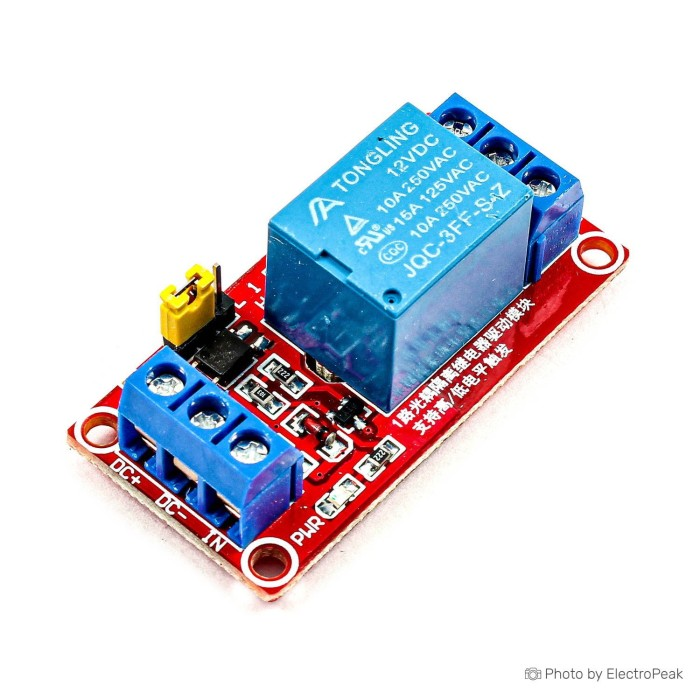
\includegraphics[width=0.48\textwidth]{resources/DomainAnalysis/HardwareComponents/relay_module.png}%
}{%
    \fbox{\parbox{0.46\textwidth}{\centering\color{gray}\small
        [Photo pending --- save to resources/DomainAnalysis/HardwareComponents/relay\_module.png]}}%
}
\caption{Relay module used as binary actuator}
\label{fig:relay_module}
\end{figure}

\begin{figure}[H]
\centering
\IfFileExists{resources/DomainAnalysis/HardwareComponents/battery_9v.png}{%
    \includegraphics[width=0.38\textwidth]{resources/DomainAnalysis/HardwareComponents/battery_9v.png}%
}{%
    \fbox{\parbox{0.36\textwidth}{\centering\color{gray}\small
        [Photo pending --- save to resources/DomainAnalysis/HardwareComponents/battery\_9v.png]}}%
}
\caption{External 9 V battery used by the relay-switched load branch}
\label{fig:battery_9v}
\end{figure}

\subsubsection{LED Indicators, Resistors, and Breadboard}

LEDs with current-limiting resistors represent the switched load states on the breadboard. The breadboard provides the temporary interconnection structure used for physical validation.

\begin{figure}[H]
\centering
\IfFileExists{resources/DomainAnalysis/HardwareComponents/led.png}{%
    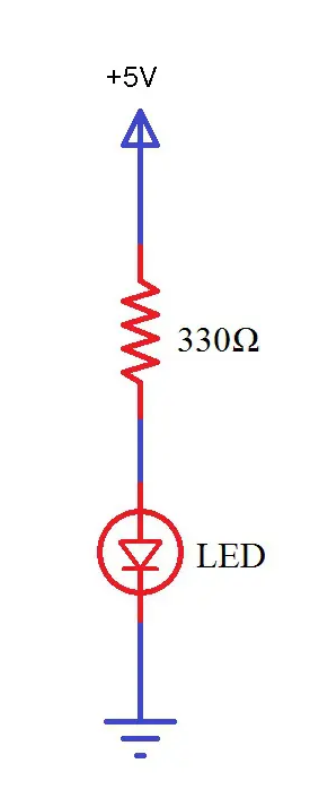
\includegraphics[width=0.38\textwidth]{resources/DomainAnalysis/HardwareComponents/led.png}%
}{%
    \fbox{\parbox{0.36\textwidth}{\centering\color{gray}\small
        [Photo pending --- save to resources/DomainAnalysis/HardwareComponents/led.png]}}%
}
\caption{LED used as relay-switched visual load}
\label{fig:led}
\end{figure}

\subsection{Software Components}

\subsubsection{PlatformIO}

PlatformIO is the build and dependency-management environment used by the repository. Lab 5.1 is added as its own environment, `lab5\_1`, so it can be built without overwriting earlier labs.

\begin{figure}[H]
\centering
\IfFileExists{resources/DomainAnalysis/SoftwareComponents/platformio.png}{%
    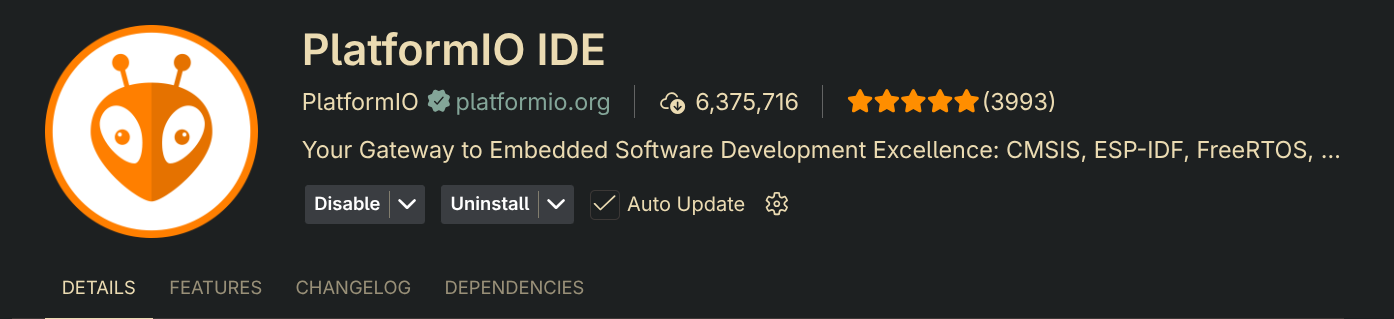
\includegraphics[width=0.75\textwidth]{resources/DomainAnalysis/SoftwareComponents/platformio.png}%
}{%
    \fbox{\parbox{0.73\textwidth}{\centering\color{gray}\small
        [Screenshot pending --- save to resources/DomainAnalysis/SoftwareComponents/platformio.png]}}%
}
\caption{PlatformIO IDE in VS Code}
\label{fig:platformio}
\end{figure}

\subsubsection{Wokwi Wiring Reference}

Wokwi is included to preserve a machine-readable circuit representation and pin map. Because this laboratory is intended to be executed on a real Arduino system, the Wokwi circuit is treated as a documentation and wiring reference rather than the primary validation environment.

\begin{figure}[H]
\centering
\IfFileExists{resources/DomainAnalysis/SoftwareComponents/wokwi.png}{%
    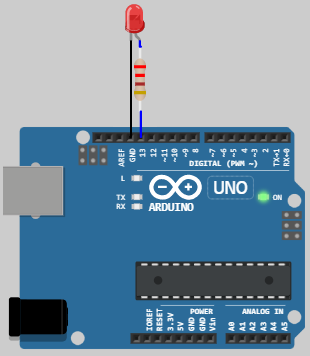
\includegraphics[width=0.75\textwidth]{resources/DomainAnalysis/SoftwareComponents/wokwi.png}%
}{%
    \fbox{\parbox{0.73\textwidth}{\centering\color{gray}\small
        [Screenshot pending --- save to resources/DomainAnalysis/SoftwareComponents/wokwi.png]}}%
}
\caption{Wokwi environment used as wiring reference}
\label{fig:wokwi}
\end{figure}

\subsection{System Architecture and Justification}

The architecture separates the control system into application orchestration, service-level control logic, reusable ECAL wrappers, and low-level Arduino libraries. This separation keeps the lab-specific code focused on task scheduling and state flow, while drivers such as LCD, keypad, relay, DHT22, and analog setpoint reading remain reusable.

The DHT22 is intentionally sampled every 2000 ms, because the sensor is not designed for high-rate acquisition. The control and relay actuation tasks are event-driven by semaphores, so the actuator reacts immediately after a new valid measurement is processed. The display task runs faster than the acquisition task in order to keep keypad entry and state changes visible on the LCD.

\subsection{Case Study - Relevant Applicability of the Solution}

ON-OFF control with hysteresis is common in thermostats, incubators, greenhouse ventilation, refrigeration systems, and pump control. In each case, the actuator usually has mechanical or thermal inertia, making frequent switching undesirable. Hysteresis protects relay contacts, reduces audible and electrical noise, and produces stable behavior with minimal computational cost. The same design pattern can be adapted from temperature regulation to humidity control, liquid-level control, fan triggering, and industrial alarm thresholds.
